% Copyright (c) 2013 by the University of Waikato, Hamilton, NZ. 
% This work is made available under the terms of the 
% Creative Commons Attribution-ShareAlike 3.0 license, 
% http://creativecommons.org/licenses/by-sa/3.0/. 
%
% Version: $Revision$

\documentclass[a4paper]{book}

\usepackage{wrapfig}
\usepackage{graphicx}
\usepackage{hyperref}
\usepackage{multirow}
\usepackage{scalefnt}
\usepackage{tikz}

% watermark -- for draft stage
\usepackage[firstpage]{draftwatermark}
\SetWatermarkLightness{0.9}
\SetWatermarkScale{5}

% Copyright (c) 2009 by the University of Waikato, Hamilton, NZ. 
% This work is made available under the terms of the 
% Creative Commons Attribution-ShareAlike 3.0 license, 
% http://creativecommons.org/licenses/by-sa/3.0/. 
%
% Version: $Revision: 2916 $

\newenvironment{tight_itemize}{
\begin{itemize}
  \setlength{\itemsep}{1pt}
  \setlength{\parskip}{0pt}
  \setlength{\parsep}{0pt}}{\end{itemize}
}

\newenvironment{tight_enumerate}{
\begin{enumerate}
  \setlength{\itemsep}{1pt}
  \setlength{\parskip}{0pt}
  \setlength{\parsep}{0pt}}{\end{enumerate}
}

% if you just need a simple heading
% Usage:
%   \heading{the text of the heading}
\newcommand{\heading}[1]{
  \vspace{0.3cm} \noindent \textbf{#1} \newline
}

\newcommand{\icon}[1]{\tikz[baseline=-3pt]\node[inner sep=0pt,outer sep=0pt]{\includegraphics[height=1.1em]{#1}};}


\title{
  \textbf{ADAMS} \\
  {\Large \textbf{A}dvanced \textbf{D}ata mining \textbf{A}nd \textbf{M}achine
  learning \textbf{S}ystem} \\
  {\Large Module: adams-nlp} \\
  \vspace{1cm}
  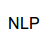
\includegraphics[width=2cm]{images/nlp-module.png} \\
}
\author{
  Peter Reutemann
}

\setcounter{secnumdepth}{3}
\setcounter{tocdepth}{3}

\begin{document}

\begin{titlepage}
\maketitle

\thispagestyle{empty}
\center
\begin{table}[b]
	\begin{tabular}{c l l}
		\parbox[c][2cm]{2cm}{\copyright 2013} &
		\parbox[c][2cm]{5cm}{
\includegraphics[width=5cm]{images/coat_of_arms.pdf}} \\
	\end{tabular}
	
\includegraphics[width=12cm]{images/cc.png} \\
\end{table}

\end{titlepage}

\tableofcontents
\listoffigures
%\listoftables

%%%%%%%%%%%%%%%%%%%%%%%%%%%%%%%%%%%
\chapter{Introduction}
\textit{The Stanford Parser} is a GPL-licensed\footnote{version 2 or later \url{http://www.gnu.org/licenses/gpl-2.0.html}{}} 
library for natural language parsing.

\noindent For instance, parsing this sentence:
\begin{verbatim}
  The quick brown fox jumps over the lazy dog
\end{verbatim}
will result in a parse tree like this:
\begin{verbatim}
  (ROOT (NP (NP (DT The) (JJ quick) (JJ brown) (NN fox)) (NP (NP (NNS jumps)) 
    (PP (IN over) (NP (DT the) (JJ lazy) (NN dog))))))
\end{verbatim}
The same parse tree in graphical representation:
\begin{figure}[htb]
  \centering
  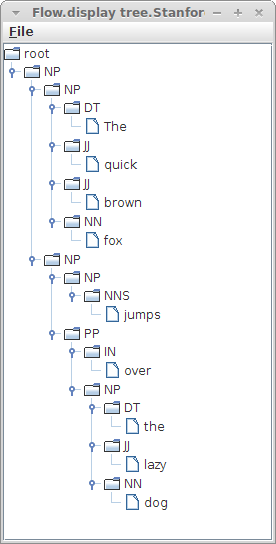
\includegraphics[width=4.0cm]{images/parse-tree.png}
  \caption{Graphical representation of Stanford parse tree.}
  \label{parse-tree}
\end{figure}

%%%%%%%%%%%%%%%%%%%%%%%%%%%%%%%%%%%
\chapter{Flow}
The following actors are available:
\begin{tight_itemize}
	\item \textit{DocumentToSentences} -- transformer for splitting document 
	strings into sentences using a specified 
	splitter/tokenizer.\footnote{adams-nlp-split\_document\_and\_parse.flow}
	\item \textit{StanfordGrammaticalStructure} -- transformer for generating a 
	grammatical structure from a parse tree.\footnote{adams-nlp-parse.flow}
	\item \textit{StanfordLexicalizedParser} -- transformer for generating a 
	parse tree from a string.\footnote{adams-nlp-parse.flow}
	\item \textit{StanfordParseTreeDisplay} -- sink for displaying a parse 
	tree.\footnote{adams-nlp-parse.flow}
\end{tight_itemize}
The following conversions are available:
\begin{tight_itemize}
    \item \textit{StanfordParseTreeToSpreadSheet} -- turns the leaves of a
    parse tree into a spreadsheet.
	\item \textit{StanfordParseTreeToXML} -- turns a parse tree into an 
	XML string.\footnote{adams-nlp-parse.flow}
\end{tight_itemize}

%%%%%%%%%%%%%%%%%%%%%%%%%%%%%%%%%%%
% Copyright (c) 2009-2012 by the University of Waikato, Hamilton, NZ. 
% This work is made available under the terms of the 
% Creative Commons Attribution-ShareAlike 4.0 license,
% http://creativecommons.org/licenses/by-sa/4.0/.
%
% Version: $Revision$

\begin{thebibliography}{999}
	% to make the bibliography appear in the TOC
	\addcontentsline{toc}{chapter}{Bibliography}

    % references
	\bibitem{adams}
		\textit{ADAMS} -- Advanced Data mining and Machine learning System \\
		\url{https://adams.cms.waikato.ac.nz/}{}
		
	\bibitem{dl4j}
		\textit{deeplearning4j} -- open-source, distributed,
		deep-learning library for the JVM. \\
		\url{http://deeplearning4j.org/}{}

	\bibitem{json}
		\textit{JSON} -- JavaScript Object Notation is a lightweight data-interchange format \\
		\url{http://json.org/}{}

	\bibitem{yaml}
		\textit{YAML} -- is a human friendly data serialization
                standard for all programming languages. \\
		\url{http://yaml.org/}{}

\end{thebibliography}


\end{document}
